%%%%%%%%%%%%%%%%%%%%%%%%%%%%%%%%%%%%%%%%%%%%%%%%%%%%%%%%%%%%%%%%%%%%%%%%%%%%%%%%
\begin{abstract}
	\noindent \textbf{Estimating music similarity by merging various similarity measurements of timbral, melodic and rhythmic features of the music with the help of the big data framework Spark.}\\
	This thesis is about the comparison of construction noise and modern-day music. 
	The field of music information retrieval (MIR) in computer science is mostly a data-driven and purely mathematical topic. The goal of this thesis is to merge the fields of computer science with music-theoretical knowledge and to find potential weak spots of current music similarity algorithms focusing on single aspects like melody, rhythm, and timbre. 

\end{abstract}

%----------------------------------------------------------------------------------------
%	THESIS CONTENT - CHAPTERS
%----------------------------------------------------------------------------------------

\mainmatter % Begin numeric (1,2,3...) page numbering
\pagenumbering{arabic}

%%%%%%%%%%%%%%%%%%%%%%%%%%%%%%%%%%%%%%%%%%%%%%%%%%%%%%%%%%%%%%%%%%%%%%%%%%%%%%%%
\chapter{Introduction}\label{intro}

The idea originated from Dr. T. Bosse from the chair for advanced computing at the Friedrich-Schiller-University (FSU) in Jena. When proposing the idea for a master thesis with the topic of "Music similarity measurement using genre-specific features" using different guitar play styles in modern-day metal music, he jokingly said that he would also like to know how metal music compares to construction building noise. The idea is actually not so groundless, considering that most people would agree on the fact that metal music is often described as noise by people not used to listening to genres like death and black metal.
While refining the original idea of the theme for this master's thesis and during the first tests, it became obvious, that while there is a lot of research in the area of music similarity for single aspects of music like melody or rhythm, there was no attempt to 



%This thesis is meant to evaluate how music similarity algorithms compare construction noise to common musical genres and how to possibly improve these algorithms.

\section{Why and How?}

\underline{Why is music similarity research even necessary?} 
\ \\
\ \\
With music streaming services like Spotify, Amazon Music, Deezer or Tidal and music sharing websites like SoundCloud, access to millions of songs is giving. To explore this humongous amount of data, the need for music recommender systems rises. SoundCloud Go+, the streaming service of SoundCloud alone gives access to more than 135 million songs \cite{bibid}. 
Of course the streaming platforms are aware of these challenges. When using services like "[ . . . ] Spotify Radio, iTunes Radio, Google Play Access All Areas and Xbox Music. Recommendations are typically made using (undisclosed) content-based retrieval techniques, collaborative filtering data or a combination thereof." \cite[p. 9]{knees1}
And also in academic research, a lot of work was done researching music similarity metrics for different aspects of music and some even for combinations of features. But all of these recommendation engines are fixed. Music 
 
\underline{What to improve?}

First of all, there is no fixed definition of music similarity so far. This is one of the first problems, dealing with this topic. Instead, there is a wide spectrum of multifaceted approaches using various feature sets and aspects of the music that has to be evaluated. Merging multiple approaches with different weights can offer a more diverse music recommendation system. To do this, a lot of different features would be required and have to be extracted from the audio data.\\
Content (music features) and context (listener behavior) data can then be fed into a big data framework to speed up operations.
Collecting this data for large amounts of songs results in big datasets that need to be explored efficiently.\\
\ \\


The goal of this thesis is to propose a transparent music similarity retrieval method based on various weighted content-based data. 
Applying different weights to different features allows similarity retrieval methods to search for different kinds of similarities. 
E.g., weighing the tempo and beat of a song more then melodic similarity allows the creation of playlists for workout and sport, whilst melodic/ timbre, etc. similarities allows to search for similar songs from musical subgenres. 
The user would get to decide what kind of playlist he wants to create. 
Adding contextual data and feeding it to an algorithm could add more or less popular music to the playlist with the goal to discover new upcoming artists or get other popular and most listened to music. 
For this thesis, however, the focus lies on content-based data/ audio features.\\ 
\ \\
\underline{How to approach this?}
\ \\
\ \\
First of all, a lot of data is required. In the first part, different scientific datasets are evaluated. 
Secondly, the available features are shown and explained. 
In the third part, different metrics are explained using the previously explored features. 
Lastly, a big data approach to efficiently use the gathered features is proposed and evaluated. A way to evaluate the results is also proposed.

\section{Overview}

\textit{Structure: \\}
\ \\
\begin{figure}[htbp]
	\centering
	%\smartdiagramset{set color list={blue!40!white, blue!40!white,blue!40!white, blue!40!white, blue!40!white}}
	\tikzset{priority arrow/.append style={rotate=180,anchor=0,xshift=30,}}
	\smartdiagram[priority descriptive diagram]{PART IV: Performance Tuning, PART III: Similarity Estimation, PART II: Feature Extraction, PART I: Data Aggregation}
\end{figure}

\section{Big Data}

Why using a big data framework would help: 
music similarity is not well defined. It is a rather subjective value that differs from listener to listener. 
Two tracks could be considered as "similar" when they are equal in tempo, loudness, melody, instrumentation, key, rhythm mood, lyrics or a combination of more than a few of these features. The usage of a big data framework allows creating a variable/ fuzzy metric definition. Various parameters could easily be taken into consideration when calculating the musical distance of two different pieces. 
Using a Big Data framework, the problem of the fuzzy definition of music similarity could be avoided, if a metric can be found, that takes multiple of the accounted features of this thesis into consideration.
Available information includes metadata, user data, audio features, sheet music, and more.

\chapter{Music Information Retrieval and Big Data}\label{audiofeat}

The field of music information retrieval (MIR) is a large research area combining studies in computer science like signal processing and machine learning with psychology and academic music study. To get started, a brief overview is given in the next section providing the most important information about publicly available datasets, MIR toolkits, and different approaches to music similarity using various audio features. An overview over big data frameworks is included as well. More in-depth information about selected metrics is later given in chapter \ref{simanal}. 

\section{Audio Features}

\subsection{Fourier Transformation}\label{featsec}

Most of the algorithms for audio data analysis start with switching from the time domain to the frequency domain, by performing a Discrete Fourier transform as described in equation \ref{eq:fft} and then computing the power spectrum (equation \ref{eq:absfft}) 
\begin{equation} \label{eq:fft}
%p (v \vert \lambda)=\sum_{i=1}^{M}w_iN(v \vert \mu_i,\sum_i) \label{prob}
X_m = \sum_{k=0}^{K-1}{x_k \cdot e^ { - \frac{K}{ 2 \cdot \pi \cdot i}\cdot k\cdot m}}
\end{equation}
\begin{equation} \label{eq:absfft}
%p (v \vert \lambda)=\sum_{i=1}^{M}w_iN(v \vert \mu_i,\sum_i) \label{prob}
|X_m| = \sqrt{Re(X_m)^2 + Im(X_m)^2}
\end{equation}
Figure \ref{laylaspec} shows the resulting spectrogram (spectrum of frequencies over time) of the first bars of the song Layla by Eric Clapton. The sound sample was recorded on an electric guitar. Since the human ear perceives sound in a non-linear matter, a logarithmic or Mel-scale fits better to represent different pitches. For example, the note A4 is perceived at a frequency of 440Hz, the A note of next octave (A5) is at 880Hz and the next one is at 1600Hz and so on. The Mel-scale was introduced to resemble the non-linear human perception of frequency (see equation \ref{eq:mel}) \cite[pp. 53f]{knees1}.
\begin{equation} \label{eq:mel}
%p (v \vert \lambda)=\sum_{i=1}^{M}w_iN(v \vert \mu_i,\sum_i) \label{prob}
m = 1127 \cdot ln(1 + \frac{f}{700})
\end{equation}
%The following plots were created with the librosa library \cite{librosa1}.
\begin{figure}[htbp]
	\centering
	\begin{subfigure}{0.5\textwidth}
		\centering
		\framebox{\parbox{2.96in}{      
		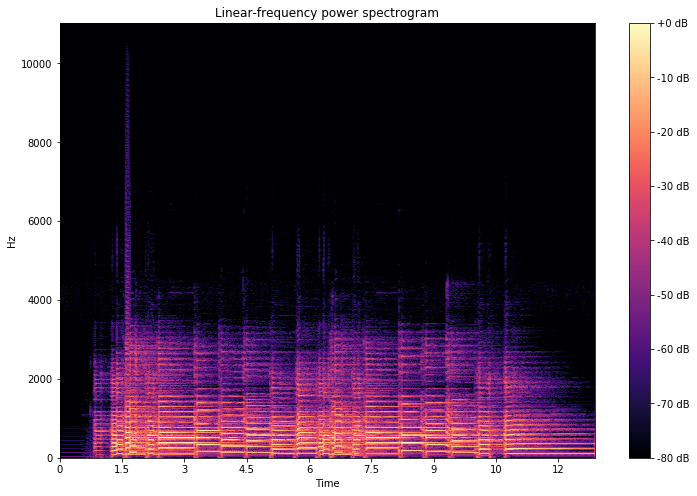
\includegraphics[scale=0.25]{Images/Layla/laylacfft.png}}}
		\captionof{figure}{Spectrogram}
		\label{laylaspec}
	\end{subfigure}%
	\begin{subfigure}{0.5\textwidth}
		\centering
		\framebox{\parbox{2.96in}{      
		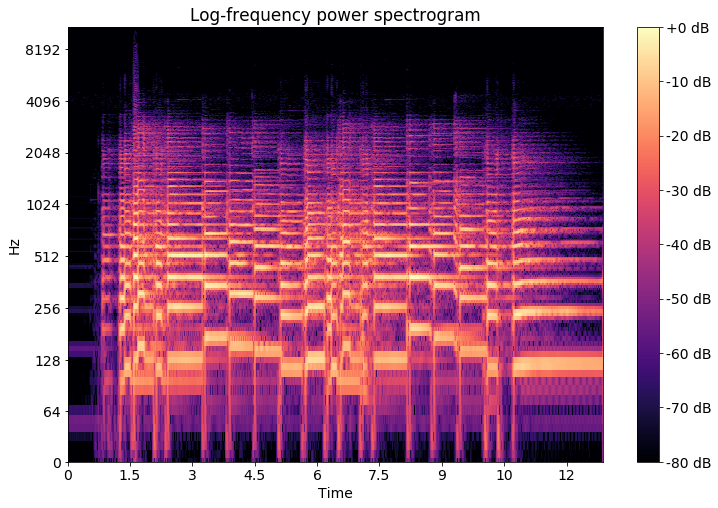
\includegraphics[scale=0.25]{Images/Layla/laylacfftlog.png}}}
		\captionof{figure}{log scaled spectrogram}
		\label{laylaspecfft}
	\end{subfigure}
	\caption{Frequency Space}
	\label{fig:test}
\end{figure}
\FloatBarrier
The high dimensionality of the spectrogram is a problem for machine learning applications and music similarity tasks, as computation based on vectors with such a high dimensionality on larger datasets would take too long for real-time applications.
Given a sample rate $f_s = 44,1kHz$ (usual CD sample-rate) and the length of a song of about $t = 180s$, the time domain contains 7938000 data points usually with 16-bit resolution for mono-channel audio. 
\begin{equation} \label{eq:points}
%p (v \vert \lambda)=\sum_{i=1}^{M}w_iN(v \vert \mu_i,\sum_i) \label{prob}
K = f_s \cdot t
\end{equation}
Calculating an FFT with a window size of 1024 samples and a hop size of 512 samples (resulting in the factor 1.5 in equation \ref{eq:hop})\cite[p. 41]{knees1}, the full, resulting spectrogram would contain 11627 frames with 1024 frequency values per frame. (eq: \ref{eq:hop}) 
\begin{equation} \label{eq:hop}
%p (v \vert \lambda)=\sum_{i=1}^{M}w_iN(v \vert \mu_i,\sum_i) \label{prob}
N_{fv} = 1.5 \cdot (\frac{44100 \ samples/s}{1024 \ samples/frame}) \cdot t
\end{equation}
To reduce the dimensionality of the feature vector, a typical approach in MIR would be to calculate the so called Mel Frequency Cepstral Coefficients (MFCCs).

\subsection{MFCCs}\label{mfccsim}

Out of all features presented in this chapter, the MFCC is the hardest one to grasp because of its abstract nature and hardly visible relatedness to musical aspects of the audio files like pitch or rhythm. This section gives a brief overview of the computation of the MFCC as stated in \cite[pp. 55ff]{knees1}.
Figure \ref{sweep} shows the magnitude spectrum of a frequency sweep signal as an example for better understanding.
\begin{figure}[htbp]
	\centering
	\framebox{\parbox{1\textwidth}{ 
	\begin{subfigure}{.495\textwidth}
		\centering 
		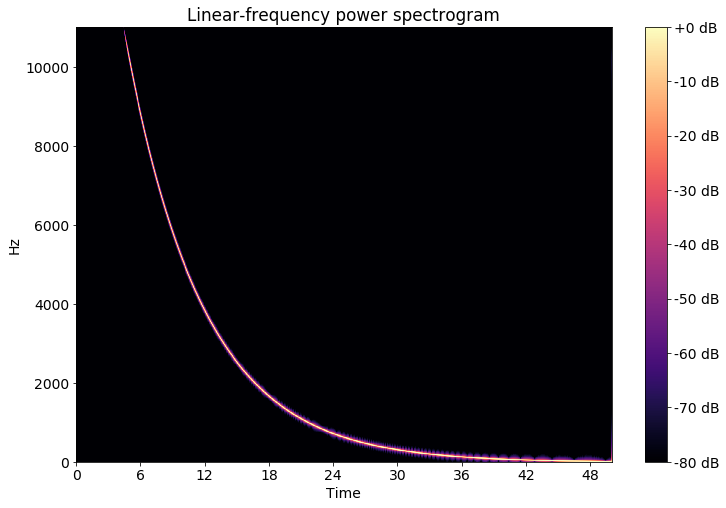
\includegraphics[scale=0.25]{Images/MFCC/sweep.png}
		\caption{Sweep signal linear}
		\label{sweeplog}
	\end{subfigure}
	\begin{subfigure}{.495\textwidth}
		\centering
		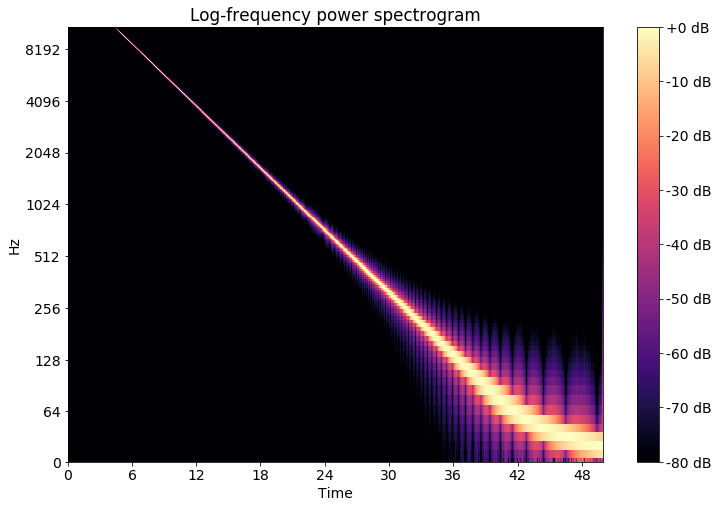
\includegraphics[scale=0.25]{Images/MFCC/sweeplog.png}
		\caption{Sweep signal logarithmic}
		\label{sweeplin}
	\end{subfigure}
	}}
	\caption{Sweep signal}	
	\label{sweep}
\end{figure}
\FloatBarrier
\noindent First of all the magnitude spectrum is transformed to the Mel-scale following equation \ref{eq:mel} by assigning each frequency value to a Mel-band.
Doing this, dimensionality reduction can be achieved by assigning multiple frequency values to one of typically 12 to 40 Mel-bands. The resulting vectors are then fed into a discrete cosine transformation (DCT) resulting in the MFCCs for each frame. 
\begin{equation} \label{eq:dct}
%p (v \vert \lambda)=\sum_{i=1}^{M}w_iN(v \vert \mu_i,\sum_i) \label{prob}
X_k = \sum_{n=0}^{N-1}{x_n cos\left[{\frac{\pi}{N}(n + \frac{1}{2})k}\right]}
\end{equation}
Figure \ref{mfcc} shows the resulting MFCCs with a high resolution of 1024 Mel bands. This is not what in a usual application would be done, because this is nearly as high-dimensional as the original spectrogram. In comparison, figure \ref{mfccs} shows the MFCC reduced to 13 Mel Bands.
To better visualize the MFCCs, all values are typically scaled to have a standard deviation of 1 and a mean value of 0 per band in the plots. 
\begin{figure}[htbp]
	\centering
	\framebox{\parbox{1\textwidth}{ 
	\begin{subfigure}{.495\textwidth}
		\centering 
		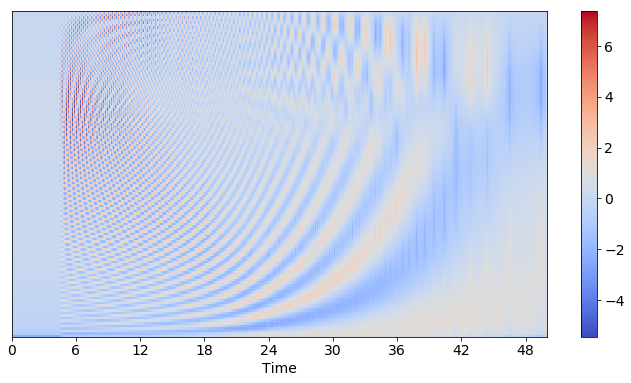
\includegraphics[scale=0.25]{Images/MFCC/mfccscaled.png}
		\caption{MFCC High Resolution}
		\label{mfcc}
	\end{subfigure}
	\begin{subfigure}{.495\textwidth}
		\centering
		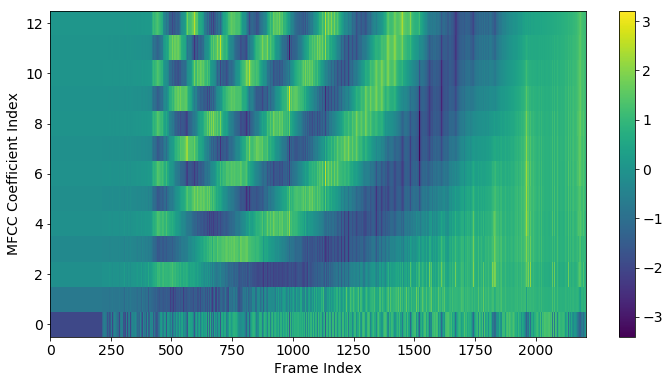
\includegraphics[scale=0.25]{Images/MFCC/mfccnorm.png}
		\caption{MFCC 12 Bands scaled}
		\label{mfccs}
	\end{subfigure}
	}}
	\caption{MFCCs}	
	\label{fig:mfcc}
\end{figure}
\FloatBarrier
MFCCs were found to be suited to represent the timbral attributes of music \cite[p. 55 ff]{knees1}. To describe a tone, three moments can be used according to \cite[pp. 15]{musicdata}: tonal intensity perceived as loudness, the tonal quality perceived as the pitch and the timbre or tonal color as the third moment. Looking at an example melody line played on a electric distorted guitar and a piano, distinct differences can be seen. Due to the physical properties of a string, every note played consists of the main frequency (the actually played key) and so-called harmonic overtones because of the way a string, e.g. in a piano, vibrates and the wooden body resonates. Typically the overtones of a piano consist of the main key, the same key a few octaves higher and major thirds and fifths of the octave. Depending on the instrument, these harmonics decline faster or slower or don't appear at all. An electrically amplified guitar amplifies these overtones as well, which is visible in figure \ref{timbreg}.
\begin{figure}[htbp]
	\centering
	\framebox{\parbox{1\textwidth}{ 
	\begin{subfigure}{.495\textwidth}
		\centering 
		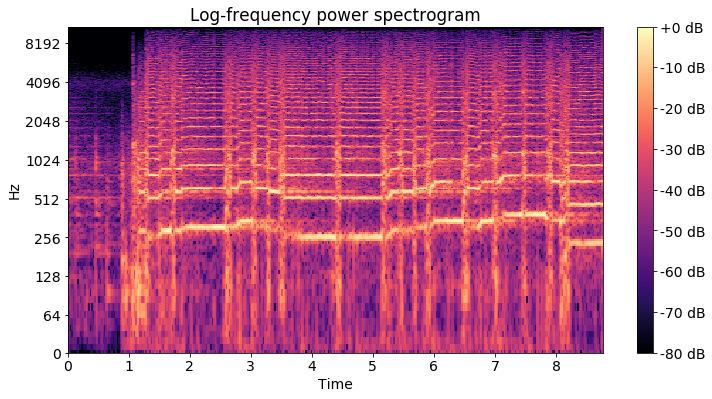
\includegraphics[scale=0.25]{Images/MFCC/timbre_eguitar.png}
		\caption{Guitar}
		\label{timbrep}
	\end{subfigure}
	\begin{subfigure}{.495\textwidth}
		\centering
		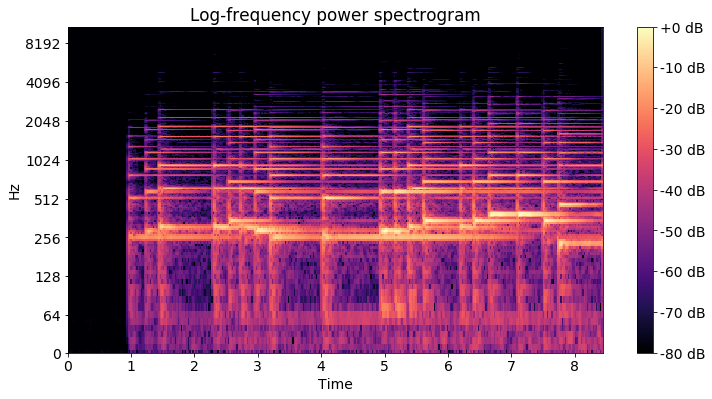
\includegraphics[scale=0.25]{Images/MFCC/timbre_piano.png}
		\caption{Piano}
		\label{timbreg}
	\end{subfigure}
	}}
	\caption{Timbre guitar vs. piano}	
	\label{fig:timbre}
\end{figure}
\FloatBarrier
These differences in timbre are also visible when looking at the MFCCs in figure \ref{fig:timbrmfcce}. This time the MFCC plots are pictured without the previously mentioned scaling. Additionally, the mean value and standard deviance of the MFCCs four to 13 are pictured in figure \ref{fig:timbrstatmfcce}. This calculation of statistical features is later explained in chapter \ref{musly}. Although both times the exact same melody is played in the same tempo, the MFCC features vary due to the different timbral properties of the instruments. 
\begin{figure}[htbp]
	\centering
	\framebox{\parbox{1\textwidth}{ 
	\begin{subfigure}{.495\textwidth}
		\centering 
		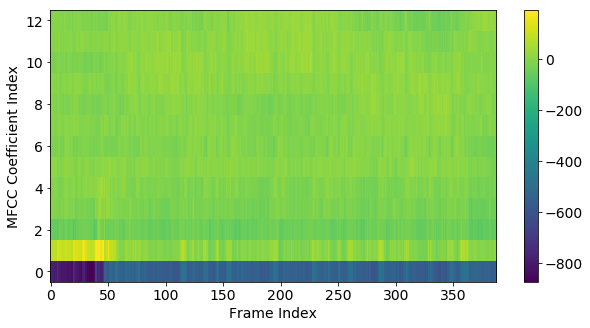
\includegraphics[scale=0.35]{Images/MFCC/mfcc_eguitar.png}
		\caption{Guitar}
		\label{mfccg}
	\end{subfigure}
	\begin{subfigure}{.495\textwidth}
		\centering
		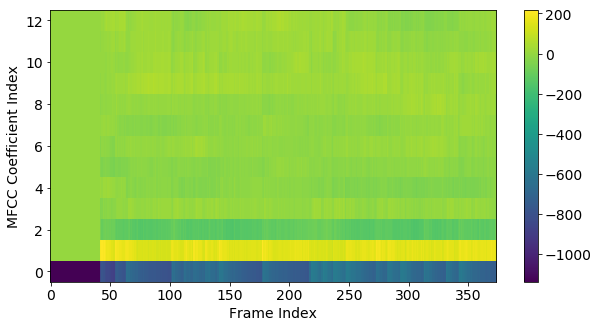
\includegraphics[scale=0.35]{Images/MFCC/mfcc_piano.png}
		\caption{Piano}
		\label{mfccp}
	\end{subfigure}
	}}
	\caption{MFCC statistics guitar vs. piano}	
	\label{fig:timbrmfcce}
\end{figure}
\FloatBarrier

\begin{figure}[htbp]
	\centering
	\framebox{\parbox{1\textwidth}{ 
	\begin{subfigure}{.495\textwidth}
		\centering 
		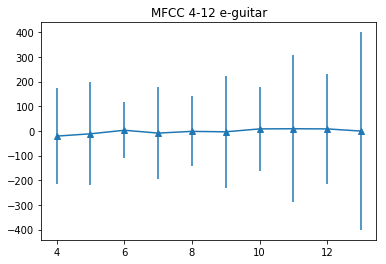
\includegraphics[scale=0.45]{Images/MFCC/stat_eguitar.png}
		\caption{Guitar}
		\label{mfccsg}
	\end{subfigure}
	\begin{subfigure}{.495\textwidth}
		\centering
		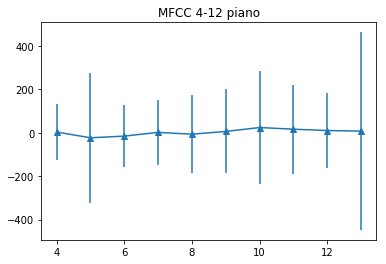
\includegraphics[scale=0.45]{Images/MFCC/stat_piano.png}
		\caption{Piano}
		\label{mfccsp}
	\end{subfigure}
	}}
	\caption{MFCC statistics guitar vs. piano}	
	\label{fig:timbrstatmfcce}
\end{figure}
\FloatBarrier

\subsection{Other Audio Features}

As another, better comprehensible, higher-level set of features, the chromagram represents the melodic/ harmonic properties of a song. The chroma plot shows the distribution of the different pitches mapped to the various semi-tones in one octave (see Figure \ref{laylachroma}). The values of each time frame are normalized to one by the strongest dimension. So if all values are close to one, it is most likely that there is only noise or silence at that frame in the recording, as depicted in the first frames of figure \ref{laylachroma}. The chromagram has one significant downside because it is reduced to one octave and thus can not represent the melody of a song to its full extent.\\
Figure \ref{laylapitch} shows the pitch curve of the recording. None but the most dominant frequencies are shown. Pitches below a certain threshold are filtered out. In contrast to the chromagram the pitch curve provides information over the whole spectrum and is not limited to one octave. These Pitch curves can be used to estimate and transcribe musical notes from audio data as presented in \ref{midiest}.\\
The low-level rhythmic features of a song include the estimation of the overall tempo, beats, and onset events. 
The Plot in figure \ref{laylacbeat} depictures the onsets and estimated beats in the first 10 seconds from a recording of the song Layla by Eric Clapton.
\begin{figure}[htbp]
	\centering
	\framebox{\parbox{1\textwidth}{ 
			\begin{subfigure}{.495\textwidth}
				\centering 
				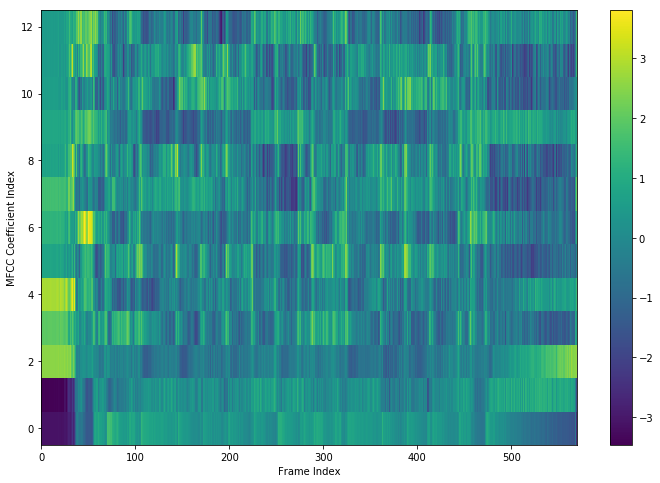
\includegraphics[scale=0.28]{Images/Layla/laylacmfcc.png}
				\caption{MFCC}
				\label{laylacmfcc}
			\end{subfigure}%
			\begin{subfigure}{.495\textwidth}
				\centering    
				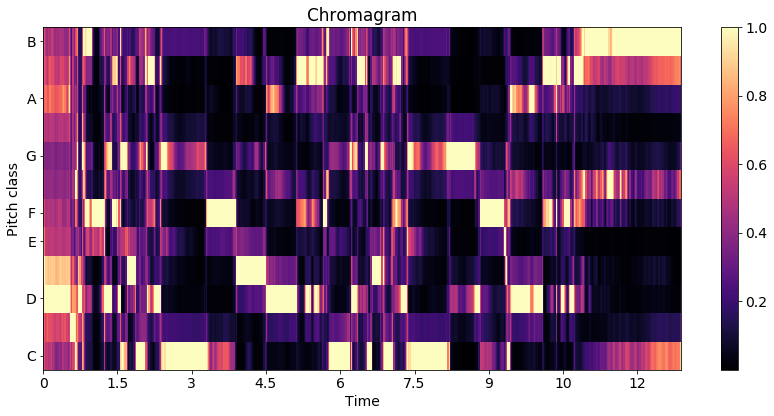
\includegraphics[scale=0.28]{Images/Layla/laylachroma.png}
				\caption{Chroma Features}
				\label{laylachroma}
			\end{subfigure}%
	}}
	\caption{Features of the song Layla by Eric Clapton}
	\label{fig:feat1}
\end{figure}

\FloatBarrier
\begin{figure}[htbp]
	\centering
	\framebox{\parbox{1\textwidth}{ 			
			\begin{subfigure}{.495\textwidth}
				\centering
				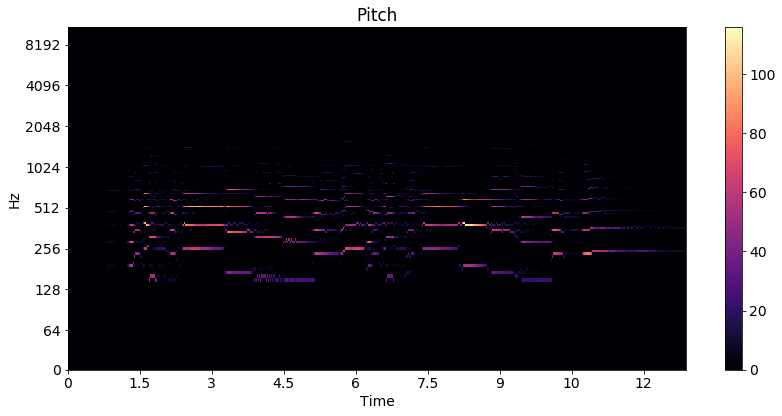
\includegraphics[scale=0.28]{Images/Layla/laylapitch.png}
				\caption{Pitch}
				\label{laylapitch}
			\end{subfigure}%
			\begin{subfigure}{.495\textwidth}
				\centering     
				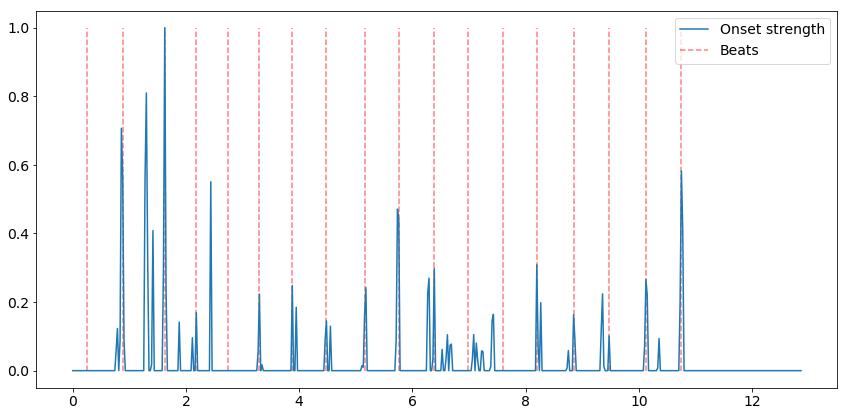
\includegraphics[scale=0.26]{Images/Layla/laylabeat.png}
				\caption{Rhythm/ Beat}
				\label{laylacbeat}
			\end{subfigure}%
	}}
	\caption{Features of the song Layla by Eric Clapton}
	\label{fig:feat2}
\end{figure}
\FloatBarrier

\section{MIR Toolkits}\label{mirtoolkit}

\subsection{Low-Level Audio Feature Extraction}
To extract audio features like the ones presented in section \ref{featsec} (MFCCs, chromagram, beats, onsets), a wide variety of toolkits is publicly available, a few are presented in \cite{audiofeattoolb}.
The YAAFE toolkit \cite{yaafe1} is able to extract a lot of different audio features like energy, MFCC, or loudness directly into the Hadoop file format *.h5 making it ideal for big data frameworks to use. It can be used with C++, Python, or Matlab.\\
The Essentia toolkit \cite{essentia1} is pretty similar to YAAFE, extending it by the calculation of rhythm descriptors, bpm, etc. It can also be used with C++ and Python\\
The Librosa Toolkit provides similar functionality \cite{labrosa1} as Essentia. It is user-friendly, well documented, and can be called from a Jupyter-Notebook \cite{jupyter}, allowing rapid prototyping and testing of different algorithms. Most of the plots in this chapter were created using librosa. Code snippets for the extraction of low-level features with Essentia and librosa is given in chapter \ref{simmet} as well as a performance analysis of both.\\

\subsection{Music Similarity}

An easy way to test state-of-the-art music similarity algorithms is to use the open-source toolkit Musly \cite{musly1}. It is based on statistical models of MFCC features and calculates the distances between songs very fast, supporting OpenMP acceleration. It automatically extracts the features it requires from the audio files. To compare the extracted features and calculate the distances, it implements the method introduced by Mandel-Ellis \cite{mandelellis1} and a timbre based improved version of the Mandel-Ellis algorithm using a Jensen-Shannon-like divergence \cite{musly2}. More details and a re-implementation of some of the features from this toolkit are presented in chapter \ref{musly}\\
As another option, the MIR Toolkit \cite{mirtoolbox1} is a toolbox for Matlab \cite{matl1}. A port to GNU Octave \cite{octave1} is also available \cite{mirtoolbox2}. The code snippet \ref{lst:MIRmat} is all it takes to compute a similarity matrix based on MFCC features, but the calculation is rather slow.

\lstset{language=Matlab}          % Set your language (you can change the language for each code-block optionally)
%\newpage
\FloatBarrier

\begin{lstlisting}[frame=single,label={lst:MIRmat},
caption={MIR Toolkit Similarity},captionpos=b]  % Start your code-block
numfiles = 326;
mydata = cell(1, numfiles);
for k = 1:numfiles
	myfilename = sprintf('%d.wav', k);
	mydata{k} = mirmfcc(myfilename);
	close all force
endfor
simmat = zeros(numfiles,numfiles);
for k = 1:numfiles
	for l = 1:numfiles
		simmat(k, l) = mirgetdata( ...
		mirdist(mydata{k}, ...
		mydata{l}));
	endfor
endfor
\end{lstlisting}
\FloatBarrier

\subsection{Melody/ Pitch Extraction}\label{midiest}
To test the various pitch extraction toolkits, one piece by Rachmaninoff and one composed by Beethoven was used. The first three bars of Rachmaninoff's Prelude in C Sharp Minor can be found in figure \ref{rm}. Figure \ref{fe} shows the first five bars of Beethoven's Bagatelle in A Minor ("Für Elise").
\begin{figure}[htbp]
	\centering
	\framebox{\parbox{1\textwidth}{ 
	\begin{subfigure}{0.5\textwidth}
		\centering      
		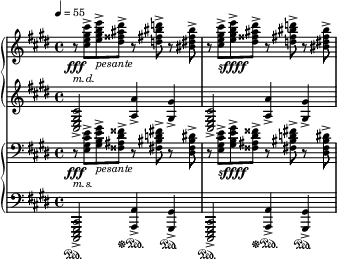
\includegraphics[scale=0.25]{Images/rachm.png}
		\caption{Rachmaninoff Prelude in C Sharp Minor \cite{rm1}}
		\label{rm}
	\end{subfigure}%
	\begin{subfigure}{0.5\textwidth}
		\centering 
		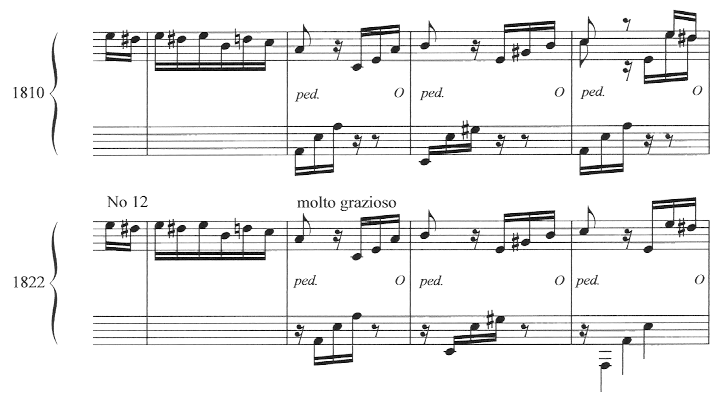
\includegraphics[scale=0.4]{Images/felise.png}
		\caption{Für Elise \cite{fe1}}
		\label{fe}
	\end{subfigure}
	}}
	\caption{Original Scores}
	\label{fig:sheets}
\end{figure}
The first toolkit tested is called aubio \cite{aubio1}. The result can be seen in figure \ref{fea} and figure \ref{raa}. The upper subplot shows the waveform of the first few seconds of each piece. The second subplot figures the estimated pitch with green dots. If the pitch is zero, then no pitch can be estimated, most likely because the associated frame contains silence. The blue dots resemble the estimated pitches where the confidence (shown as the blue graphs in the third subplot) is above a certain threshold (the orange lines in the third subplots).
\begin{figure}[htbp]
	\centering
	\framebox{\parbox{1\textwidth}{ 
	\begin{subfigure}{0.5\textwidth}
		\centering      
		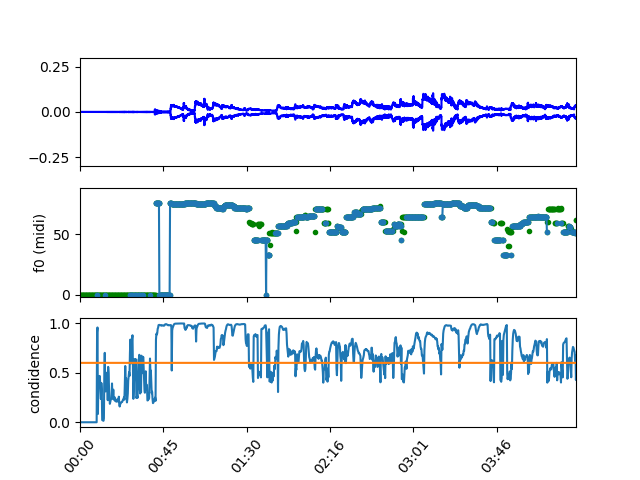
\includegraphics[scale=0.4]{Images/feliseaubio.png}
		\caption{Für Elise Aubio Pitch}
		\label{fea}
	\end{subfigure}%
	\begin{subfigure}{0.5\textwidth}
		\centering 
		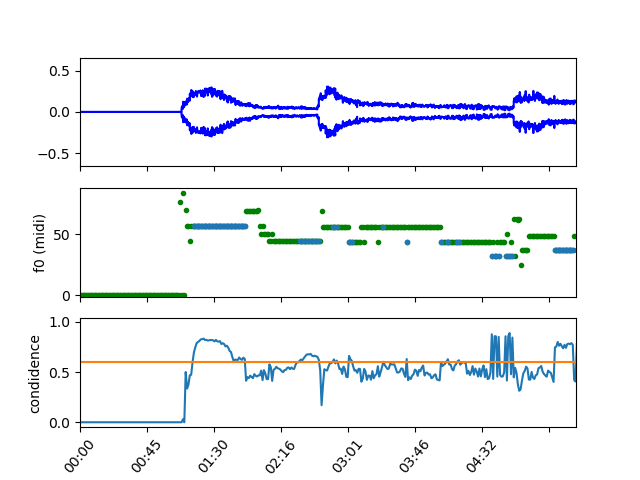
\includegraphics[scale=0.4]{Images/rachaubio.png}
		\caption{Rachmaninoff Prelude Aubio Pitch}
		\label{raa}
	\end{subfigure}
	}}
	\caption{Aubio}
	\label{fig:aubio}
\end{figure}
\FloatBarrier
The other melody extraction tool is called Melodia \cite{melodia1}, which is available as a VAMP plugin and can be used together with the Sonic Visualizer \cite{sonviz1}.\\
The results are shown in figure \ref{fem} and \ref{ram}.
The purple line is the estimated pitch; however, there are unwanted jumps between different octaves of the harmonics. 

\begin{figure}[htbp]
	\centering
	\framebox{\parbox{1\textwidth}{ 
	\begin{subfigure}{0.5\textwidth}
		\centering      
		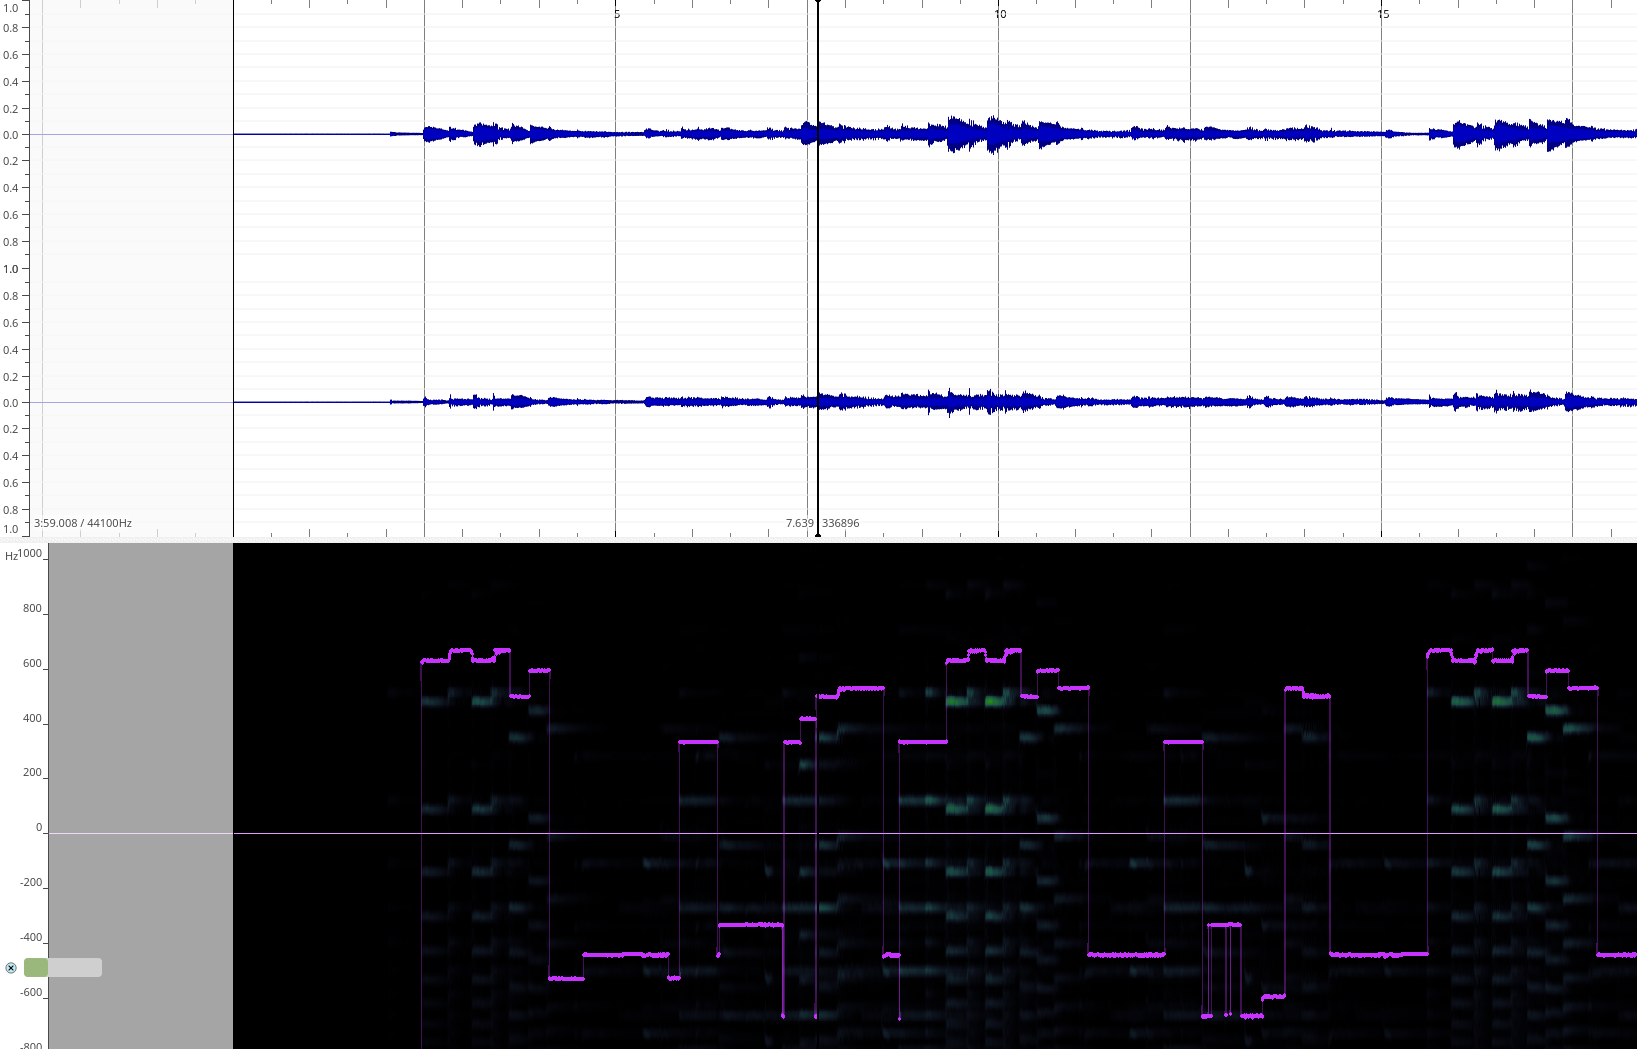
\includegraphics[scale=0.13]{Images/femelodia.png}
		\caption{Für Elise Melodia Pitch}
		\label{fem}
	\end{subfigure}%
	\begin{subfigure}{0.5\textwidth}
		\centering 
		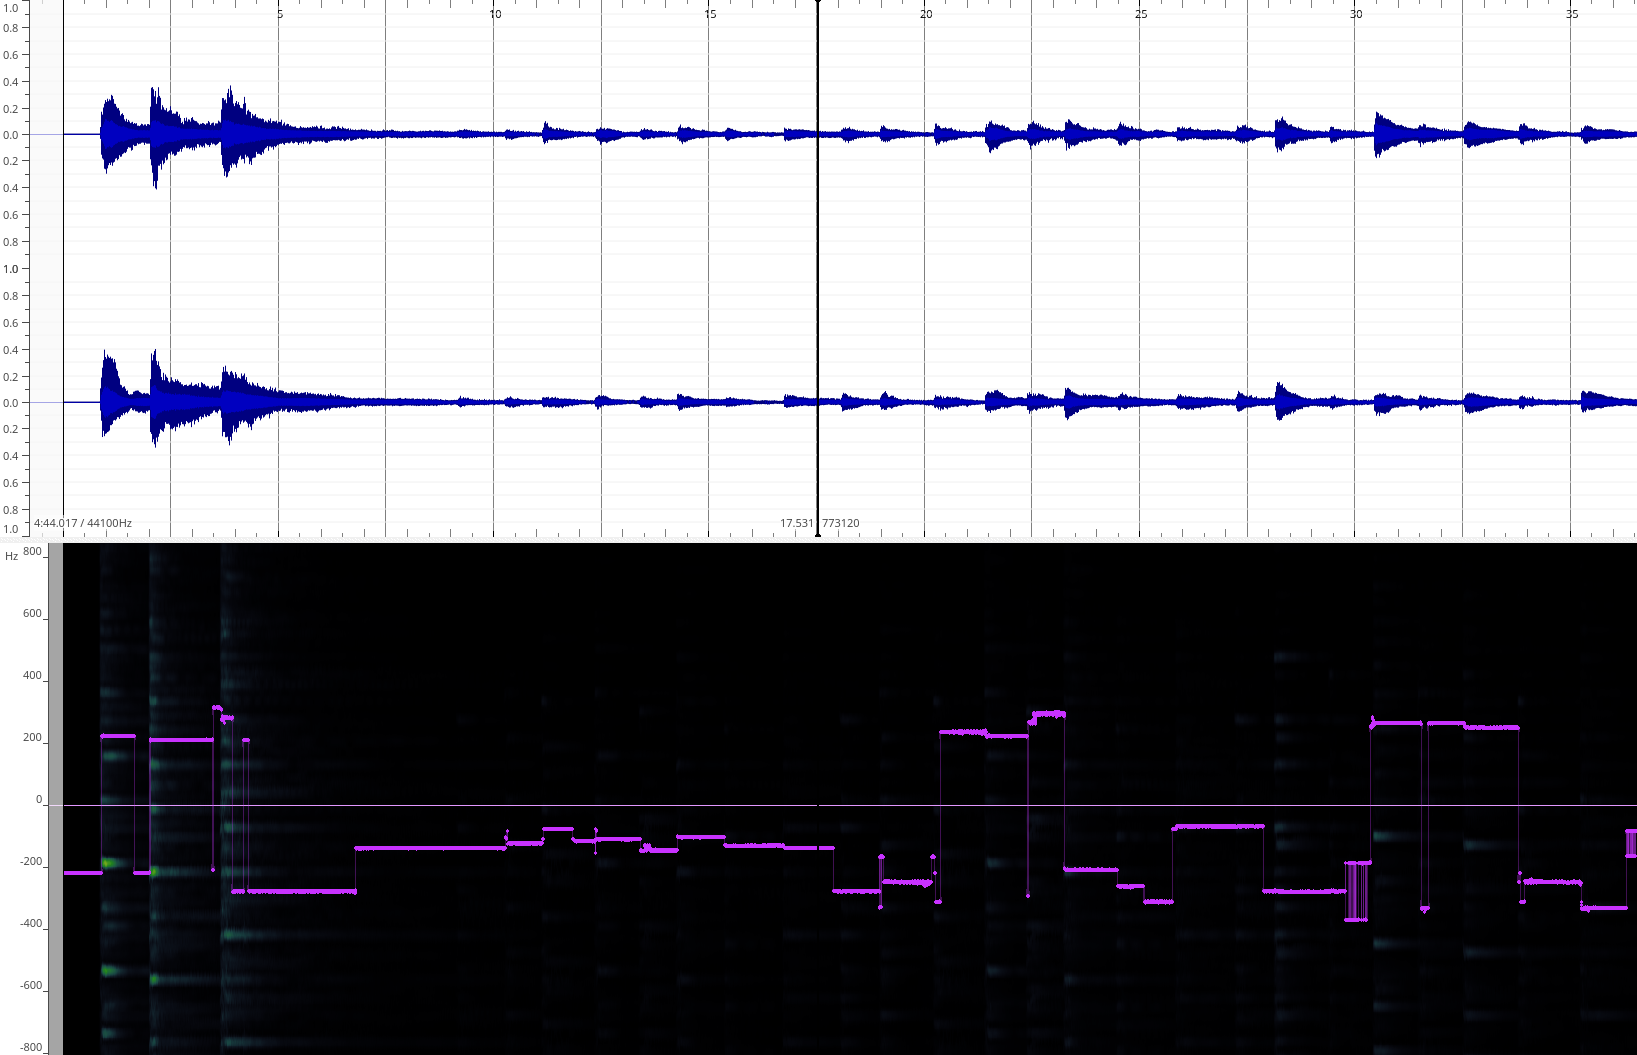
\includegraphics[scale=0.13]{Images/rmmelodia.png}
		\caption{Rachmaninoff Melodia Pitch}
		\label{ram}
	\end{subfigure}
	}}
	\caption{Melodia}
	\label{fig:melodia}
\end{figure}

\noindent Sadly the conversion from the extracted pitches to MIDI notes does not work flawlessly. It is apparent in figure \ref{fig:transc} that the transcription does not work accurately enough, even for a classical music piece with only one instrument. Figure \ref{femm} shows the output of a python script using the Melodia VAMP plugin to calculate a MIDI file containing the main melody line, and figure \ref{feam} shows the transcribed MIDI notes from Aubio. The detected melody lines are jumping between different octaves, and finding the right threshold for the separation between silence and detected notes turns out to be problematic as well.

\begin{figure}[htbp]
	\centering
	\framebox{\parbox{1\textwidth}{ 
	\begin{subfigure}{0.5\textwidth}
		\centering      
		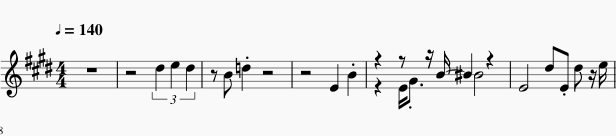
\includegraphics[scale=0.35]{Images/femelodiamidi.png}
		\caption{Für Elise Melodia MIDI}
		\label{femm}
	\end{subfigure}%
	\begin{subfigure}{0.5\textwidth}
		\centering 
		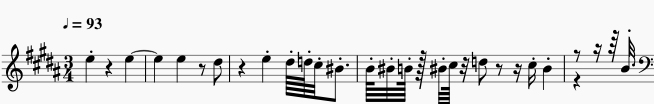
\includegraphics[scale=0.33]{Images/feam.png}
		\caption{Für Elise Aubio MIDI}
		\label{feam}
	\end{subfigure}
	}}
	\caption{Transcription}
	\label{fig:transc}
\end{figure}
\FloatBarrier 

\section{Music Similarity Measurements}

\subsection{Timbre Based}

The proposed approach by Dominik Schnitzer \cite{schnitzer1}, the creator of the Musly toolkit introduced earlier, is, to take MFCCs as low-level features and then compute statistical features like mean, standard deviation, and covariances of the different MFCCs to reduce dimensionality before computing the similarities. Another example for the computation of approximate nearest neighbors was published in the paper titled "Large-scale music similarity search with spatial trees" by Brian McFee and Gert Lanckriet \cite{msd4}.\\ 
A selection of different timbre based similarity measurements is evaluated later in chapter \ref{musly}.

\subsection{Pitch Based}

One proposed approach by Matija Marolt in 2006 is, to take mid-level melodic representations of audio files like the chromagram instead of high-level features like sheet music or low-level features like Gaussian mixture models of MFCCs, to compute the similarity between songs \cite{pitch1}. A more detailed analysis of this topic is given in chapter \ref{melsimc}.

\subsection{Note Based}

For comparing musical pieces by their symbolic representation (notes, tablatures, etc.) different text retrieval methods can be used. MIDI files as a digital representation of notes are a good starting point. For example Xia (et. al) uses a variation of the Levenshtein distance measurement to compute similarities between MIDI files \cite{chroma4}. 
The problem with notation based algorithms is that there are not many datasets available containing audio and MIDI information. As shown in section \ref{midiest}, the automatic transcription of notes from raw audio does not work flawlessly. There is still ongoing research to automatically annotate musical notes with the help of neural networks \cite{crepe1}.
In chapter \ref{rhythmsimc} an attempt to extract note information as text features from chromagrams and calculating the similarity by using the Levenshtein distance is shown and evaluated.

\subsection{Rhythm Based}

Rhythm based music similarity algorithms use timing information of various events as a baseline. For example low-level features like the onset and beat data from the plot in Figure \ref{laylacbeat} could be used as a starting point for rhythmic similarity retrieval. As an example, Foote (et. al) introduced a feature called the beat spectrum for the computation of rhythmic similarities. Other more recent or advanced approaches make use of the rhythm histogram, beat histogram, and rhythm patterns later evaluated in chapter \ref{rhythmsimc}.

\subsection{Metadata Based/ Collaborative Filtering}\label{collaborative}

Most of the research that combines the field of music information retrieval with big data frameworks relies on data based on the listening behaviour of many users of, e.g., music streaming platforms. In 2012 the MSD Challenge was brought to the MIR community. Researchers were challenged to give a list of song recommendations based on a large set of user data, the Million Song Dataset (MSD, see section \ref{datasets}). As an example, if user X listens a lot to artist A and B and user Y listens mostly to artist A and C, then user X could probably like artist C as well. These kinds of collective listening behavior based recommendations are called collaborative filtering and are pretty common in large music streaming services, although not necessarily representing direct musical similarity. \cite[p. 192f.]{knees1}\\
Recommendation systems based on collaborative filtering tend to propose commonly well-known artists rather than not so well-known ones, possibly biasing the resulting recommendation. On the other hand, these kinds of similarity algorithms can work very fast and efficient in a big data environment. The usage of annotations and metadata information like genre and artist based recommendations are common as well. The recommendation of songs based on lyrics and also hybrid recommendation systems that combine lyrics, metadata, and collaborative filtering are also possible.\\
However, all of these recommendation strategies are not directly based on musical features and are not evaluated further throughout this thesis. But they are a possible addition for a hybrid recommendation engine for future research. 
An example using user-based collaborative filtering is the paper "Design and Implementation of Music Recommendation System Based on Hadoop" \cite{metadat1}. 

\subsection{Genre Specific Features}

The impact of the choice of parameters for similarity measurements on different music subgenres was evaluated by Gulati (et al.) for Indian art music (Carnatic and Hindustani music) \cite{mussim1}. They state: "We evaluate all possible combinations of the choices made at each step of the melodic similarity computation discussed in Section 2.  We consider 5 different sampling rates of the melody representation, 8 different normalization scenarios, 2 possibilities of uniform time-scaling and 7 variants of the distance measures.  In total, we evaluate 560 different variants" \cite[p. 3]{mussim1}. This evaluation showed that the choice of features and parameters for music similarity measurement is a critical point. "Sampling rates do not have a significant impact for Hindustani music, but can significantly degrade the performance for Carnatic music." \cite[p. 3]{mussim1}. So using different kind of feature sets and parameters for the recommendation of songs from different genres could be an option but would go beyond the frame of this thesis.\\
As another idea, e.g., in Rock, Pop and Metal music, the analysis of different guitar playing techniques would be imaginable. Guitar tablature extraction \cite{guitext1} Toolkits could be used to extract information, whether the guitar in a song is mostly plucked or strummed, for instance. Or if there are Hammer-on/ Pull-off/ side bending or tapping techniques used. In classical music, the play style of the string section of an orchestra could be taken into consideration (staccato, pizzicato, etc.). These kinds of information could be used as a baseline for song recommandations. 
However, there is no MIR toolkit available for the estimation of play styles, so this idea would have to be evaluated in future research.

\subsection{Summary}

In this thesis, music similarity measurements based on three different types of features are evaluated. The first is based on MFCCs to represent timbral features of the songs and therefore offering a set of features to make recommendations that are similar in tone color and should be able to make recommendations inside the boundaries of different genres. The second is based on chroma features/ note information to provide a measurement of melodic similarity. With these features, the detection of cover versions should be possible. The third set of features is based on the rhythmic properties of a song. This should enable the recommendation of songs with the same tempo and rhythmic structure, and possibly also enable the recommendation of songs within the same genre.\\
The usage of MIDI files is not considered further due to the rather poor performance of automatic score extraction tools for songs with multiple instruments and melody lines, and the lack of datasets containing MIDI and audio files. Also, the melodic component of the songs is already represented by the chroma features, although that limits the representation to one or at most a few octaves.\\
Collaborative filtering is left out because it does not necessarily represent the musical features and properties, but instead the personal taste of other people. And secondly, it is left out because no fitting dataset with the required information and matching music files was found (see section \ref{data}).\\
Lastly, genre specific features are also not an option because this field is not yet very well researched, and the development of algorithms and the extraction of features would go beyond the scope of this thesis.

\section{Data Aggregation}\label{data}

To evaluate the music similarity algorithms and metrics, a lot of music data is needed.

\subsection{Datasets}\label{datasets}

\begin{figure}[htbp]
	\centering
	\framebox{\parbox{1\textwidth}{ 
	\begin{subfigure}{0.5\textwidth}
		\centering
		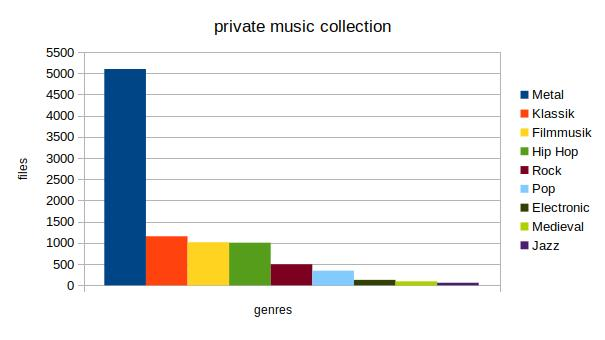
\includegraphics[scale=0.45]{Images/privmus.jpg}
		\caption{private music collection}
		\label{privmusdist}
	\end{subfigure}
	\begin{subfigure}{0.5\textwidth}
		\centering
		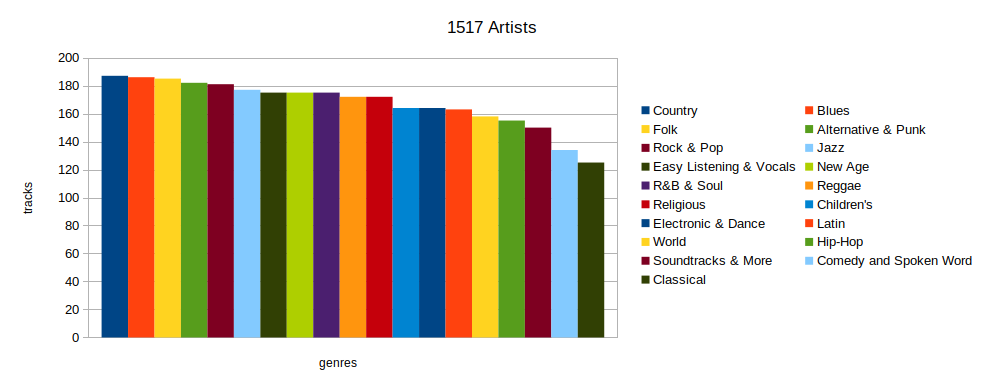
\includegraphics[scale=0.29]{Images/1517genre.png}
		\caption{1517 artists}
		\label{1517dist}
	\end{subfigure}
	
	\begin{subfigure}{0.5\textwidth}
		\centering
		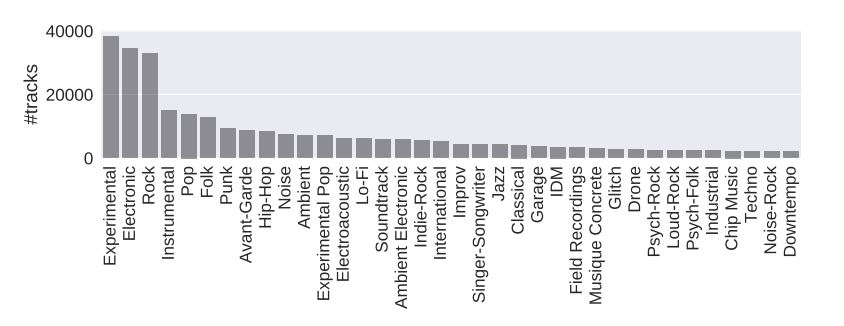
\includegraphics[scale=0.35]{Images/fma_genre.JPG}
		\caption{fma \cite[p. 4]{fma1}}
		\label{fmadist}
	\end{subfigure}
	\begin{subfigure}{0.5\textwidth}
		\centering
		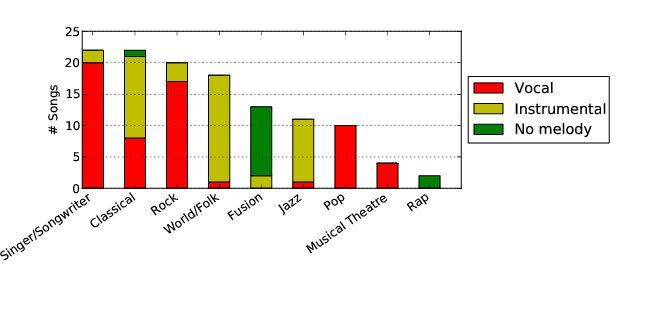
\includegraphics[scale=0.35]{Images/MedleyDB1.png}
		\caption{MedleyDB \cite[p. 2]{medleydb1}}
		\label{medleydbdist}
	\end{subfigure}
	}}
	\caption{Datasets}
	\label{fig:datasetdist}
\end{figure}
\FloatBarrier

\subsubsection{Free Music Archive}

The largest dataset is the Free Music Archive (fma) consisting of 106733 different songs totaling an amount of nearly one terabyte of music data from all kinds of different music genres \cite{fma1}. There is also a lot of metadata like genre tags available for most of the songs.

\subsubsection{Private Music Collection}

The private music collection used in this work consists mainly of metal music. The music was legally purchased; all rights belong to the respective owners. Therefore this dataset can not be published alongside this thesis. But the private music collection is fully cataloged, and the according PDF file is the appendices. The distribution of different songs per genre for this dataset is visualized in figure \ref{privmusdist}.\\
\noindent Additionally, a private recording dataset was used, consisting of ambient recordings and self-produced music. Most of these files are available on SoundCloud \cite{bqpd1}.\\
Because music recommendation is always something personal and the perception of the quality of the results may differ, the inclusion of the private music collection is necessary to enable a subjective evaluation of the results from the developed recommendation engine.

\subsubsection{1517 Artists and Musicnet}

Other sources of music are the Musicnet dataset \cite{musicnet1} and the 1517-Artists dataset \cite{1517artists1}. The Musicnet dataset includes 330 pieces of classical music with musical notes as annotations and the 1517 artists dataset contains 3180 songs of multiple genres (see figure \ref{1517dist}). 

\subsubsection{Covers80}\label{cov801}

For cover song detection analysis, the covers80 dataset is available \cite{cover80} containing eighty original songs mostly from the musical genres rock and pop and 84 cover versions. These cover versions tend to differ significantly from the original in musical style, rhythm, and timbre.\\
%The ability to detect cover songs or different versions/ recording of a musical piece could be a good measurement for the efficiency of music similarity algorithms. In the next chapter \ref{simanal}, one test case is presented, showing, that for instance an MFCC based music similarity algorithm isn't able to detect different recordings of the same piano piece as most similar to each other. 

\subsubsection{MedleyDB}

For a melody/ pitch based similarity analysis, multitrack datasets could provide useful data, because the pitch estimation can be done instrument by instrument. There is, e.g., the MedleyDB \cite{medleydb1} and MedleyDB2 \cite{medleydb2} dataset, as well as the Open Multitrack Dataset \cite{openmult1} currently consisting of 593 multitracks in which the MedleyDB dataset is already included, leaving 481 other tracks for analysis.

\subsubsection{Overview and Other Sources}

The music sources and amounts of songs used for the task at hand are listed in table \ref{table_dsets}.

\begin{table}[h]
	\begin{center}
		\begin{tabular}{|c||c|}
			\hline
			fma & 106.733 Songs\\
			\hline
			private & 8484 Songs\\
			\hline
			1517 artists & 3180 Songs\\
			\hline
			Maestro & 1184 Songs (piano) + MIDI\\
			\hline
			musicnet & 330 Songs (classical) + note annotation\\
			\hline
			Open Multitrack Testbed & 593(481) Songs/ Multitracks\\
			\hline
			covers80 & 164 Songs (80 originals + 84 covers)\\
			\hline
			MedleyDB &  122 Songs/ Multitracks\\
			\hline
			MedleyDB2 &  74 Songs/ Multitracks\\
			\hline
		\end{tabular}
	\end{center}
	\caption{music datasets}
	\label{table_dsets}
\end{table}
\FloatBarrier

\subsection{Alternatives}

\subsubsection{Spotify API/ Echonest}\label{spotipy}

Another way of getting music samples, audio features, and metadata could be by using the Spotify API \cite{spotifyapi1}.
%A part of the available audio features comes from the Echo Nest\cite{echonest1}.
The Downside using the Spotify API is that there is no packed and ready to use test dataset containing the relevant features. So for scientific purposes, a test dataset would have to be created first. With a small Python library named Spotipy, the available information can be accessed very easily. \cite{spotipy1}\\
%For the purpose of this thesis, the option of creating an own dataset using the Spotify API and Spotipy was considered and ten very small test playlists of different genres were created using the Spotify Playlist Miner \cite{spotmin1}. 
Appendix \ref{spotcrawl} lists a small script, that is able to download all audio features and analysis data from selected songs in a playlist that contain a preview URL with to 30-second audio snippet. The audio features and analysis data is saved as a JSON file containing information over:
\begin{itemize}
	\setlength\itemsep{-0.5em}
	\item acousticness
	\item danceability
	\item instrumentalness
	\item liveness
	\item loudness
	\item speechiness
	\item valence
	\item predicted key
	\item tempo 
\end{itemize}
as well as pitch and timbre information, beats, and bars.
In figure \ref{spp} the returned chroma features of the piano piece "Für Elise" by Beethoven are shown and figure \ref{spp2} shows the beginning of the piece in more detail, including green dots that resemble estimated bar markings. The blue dots represent the note values of one octave. That means they can resemble a value between zero and eleven with zero representing the key C and 11 is representing a B. The Spotify API actually returns a chroma feature value for every single one of the semi-tones per segment, with one segment being a section of samples that are relatively uniform in timbre and harmony. But in the plots, only the most dominant key per segment is shown.
\begin{figure}[htbp]
	\centering
	\framebox{\parbox{1\textwidth}{ 
	\begin{subfigure}{0.5\textwidth}
		\centering      
		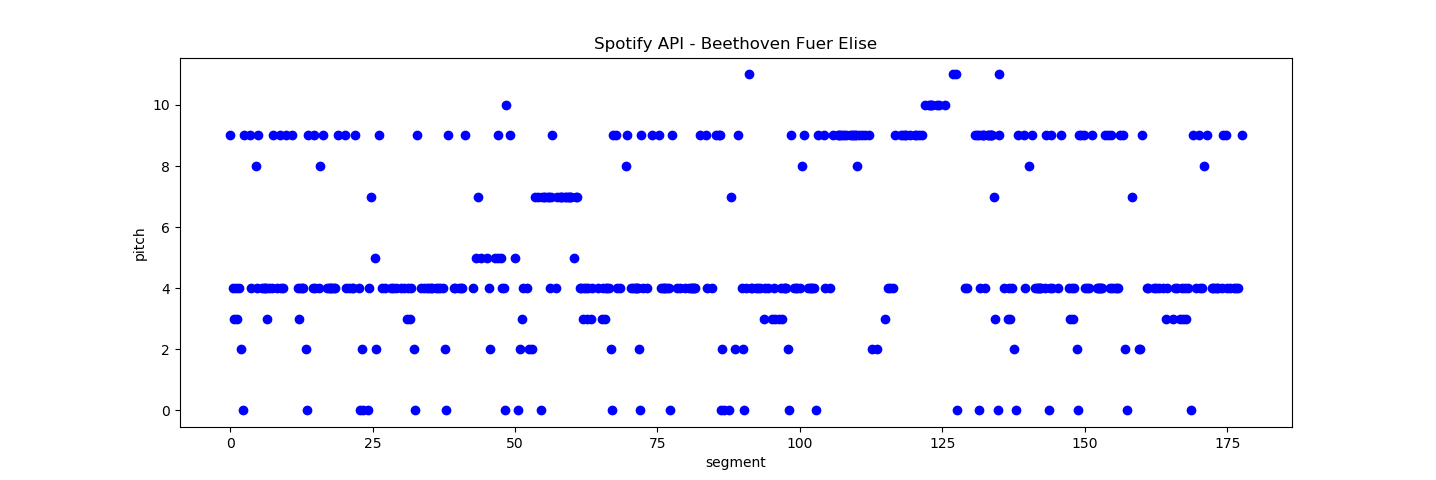
\includegraphics[scale=0.22]{Images/spot1.png}
		\caption{Für Elise Spotify pitch}
		\label{spp}
	\end{subfigure}%
	\begin{subfigure}{0.5\textwidth}
		\centering 
		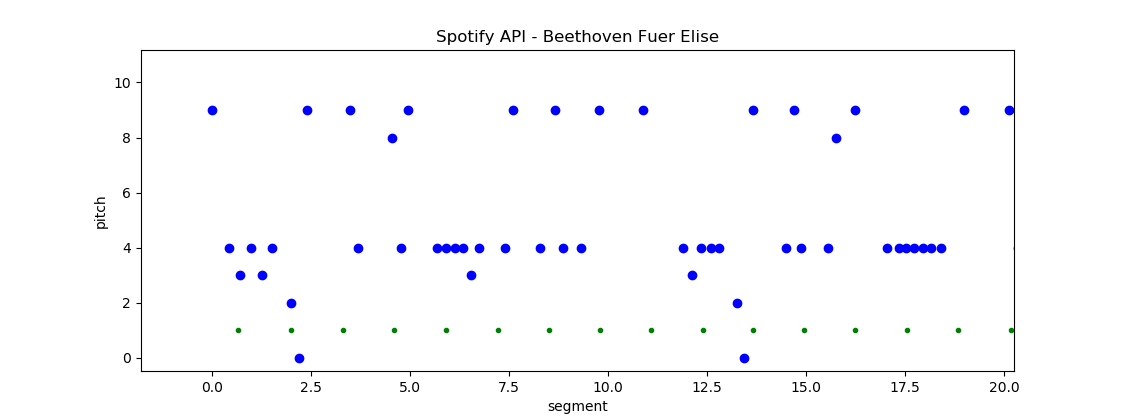
\includegraphics[scale=0.28]{Images/spot2.png}
		\caption{Für Elise detail}
		\label{spp2}
	\end{subfigure}
	}}
	\caption{Spotify API}
	\label{fig:spotify}
\end{figure}
\FloatBarrier
\ \\
Together with the 30-second audio sample from which more features like MFCCs could be extracted, Spotipy could provide all the information needed to build a large dataset for MIR. However, the terms and conditions explicitly prohibit crawling the Spotify service. As stated by the Spotify "Terms and Conditions of Use", section 9 (User guidelines):\\
"The following is not permitted for any reason whatsoever:\newline
[...]\\
12. “crawling” the Spotify Service or otherwise using any automated means (including bots, scrapers, and spiders) to view, access, or collect information from Spotify or the Spotify Service" \cite{spottac1}\\
Therefore a larger dataset based on the Spotify API can not be created without the risk of legal infringements. %Upon request the Spotify API developer team did not respond and therefore in this thesis the Spotify API wont be used to create a test dataset.\\ 
One could argue, that there is a difference between data mining and data crawling and for small datasets these restrictions may not apply.
%, when the purpose the recommendations would be the creation of Spotify playlists.\\ 
%In the sense of the Spotify Developer Terms of Service \cite{spottac2} there may be no legal infringements by creating a non-commercial playlist generation tool. 
Spotify states that by creating an algorithmically generated playlists similar to the "Discover Weekly" playlists one may run into challenges if using such features commercially \cite{spottac3}. However it does not prohibit the usage for non-commercial cases.\\ 
Upon an initial request, the Spotify API developer team did not respond and therefore in this thesis the Spotify API won't be used to create a test dataset. Without further reaching out to Spotify, using the Spotify API to create a test dataset is not an option. 

\subsubsection{Million Song Dataset}

Another outstanding and very large dataset is the Million Song Dataset (MSD)\cite{msd1}. 
It contains a large set of metadata per track as well as a lot of supplementary datasets, like the tagtraum genre annotation (figure \ref{msddist})\cite{msd5} and the Last.fm dataset\cite{msd2}. On top of that, the Echo Nest API dataset contains a lot of additional audio features like pitch, loudness, energy, and danceability to name just a few \cite{msd3}. 
Another addition is the secondhand dataset, containing a list of cover songs in the Million Song Dataset\cite{msd6}
\begin{figure}[thpb]
	\centering
	\framebox{\parbox{3in}{      
			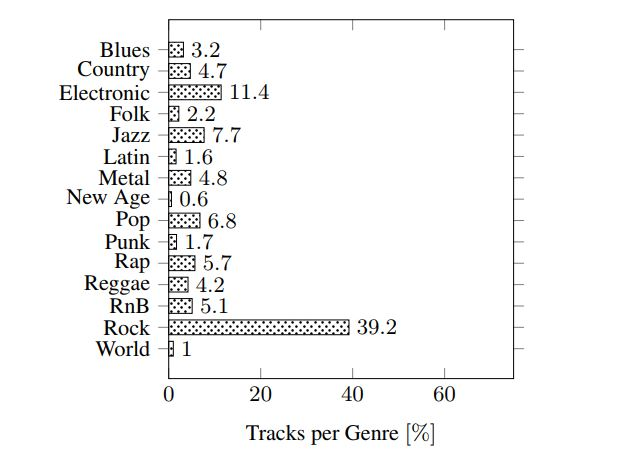
\includegraphics[scale=0.5]{Images/MSD_Tagtraum.JPG}}}
	\caption{million song dataset genre distribution \cite[p. 6]{msd5}}
	\label{msddist}
\end{figure}
\FloatBarrier
\noindent Due to the fact that the Spotify API\cite{spotifyapi1} also works with audio features from the Echo Nest\cite{echonest1}, the MSD could be used in a big data environment to simulate the work with Spotify data, without the need of mining the actual data. The MSD was already used in Big Data frameworks for music similarity retrieval based on metadata and user information (see \cite{msd4}). Although the MSD does not contain any audio files in the first place, 30-second samples could be gathered through simple scripts from 7digital.com when the dataset was made publicly available. Sadly 7digital does not offer the download of the 30-second sample files any longer, which makes this dataset unusable for this thesis, because missing audio features like MFCCs can not be computed from the audio files itself. 
